We used the belief-set game structure in order to state the surveillance objective of the agent. While in principle it is possible to solve the surveillance strategy synthesis problem on this game, this is in most cases computationally infeasible, since the size of this game is exponential in the size of the original game. To circumvent this construction we propose an abstraction-based method, that given a surveillance game structure and a partition of the set of the target's locations, yields an approximation that is sound with respect to surveillance objectives for the agent.

We will use a combination of two ways to approximate belief states. First, note that we can overapproximate the agent's current belief by considering the set of possible locations of the target returned by the sensors at that step, thus, essentially, losing some of the information about which of the locations in the returned set are actually reachable at that step. While these sets often provide a useful approximation, an abstraction based solely on the observations will in general not be able to precisely capture the agent's belief when necessary. To this end, we include a different type of approximation which allows for arbitrary precision. It is based on partitioning the set of locations into finitely many sets of locations, and using a combination of such sets to overapproximate the agent's belief. In the extreme case when each of these sets consists of a single location the abstraction is capable of precisely expressing every possible belief set. In practice, however, it is often the case that coarser partitions are sufficient for finding a winning strategy for the agent when one exists.

We begin by defining abstraction partitions and the associated abstraction and concretization functions, and then use them to define the abstract game associated with them.

\bigskip
An \emph{abstraction partition} is a family $\part = \{Q_i\}_{i=1}^n$ of subsets of $L$, $Q_i \subseteq L$ such that the following hold:
\begin{itemize}
\item $\bigcup_{i=1}^n Q_i = L$ and $Q_i \cap Q_j = \emptyset$ for all $i \neq j$;
\item For each $p \in \AP$, $Q \in \part$ and $l_a \in L$, it holds that $(l_a,l_t') \models p$ iff $(l_a,l_t'') \models p$ for every $l_t',l_t'' \in Q$.
\end{itemize}
Intuitively, these conditions mean that $\mathcal Q$ partitions the set of locations of the target, and the concrete locations in each of the sets in $\part$ agree on the value of the  propositions in $\AP$.

If $\part' =  \{Q_i'\}_{i=1}^m$ is a family of subsets of $L$ such that $\bigcup_{i=1}^m Q_i' = L$ and for each $Q_i' \in \part'$ there exists $Q_j \in \part$ such that $Q_i' \subseteq Q_j$, then $\part'$ is also an abstraction partition, and we say that $\part'$ \emph{refines} $\part$, denoted $\part' \preceq \part$.

\bigskip

For $\part = \{Q_i\}_{i=1}^n$,  we define a function $\alpha_\part : L \to \part$ by $\alpha(l_t) = Q$ that maps $l_t \in L$ to the unique $Q \in \part$ with $l_t \in Q$. 

\smallskip 

We additionally define
\begin{itemize}
    \item the \emph{abstraction function}  $\alpha_{\part} : \mathcal{P}(L) \to \mathcal{P}(\part)$ by 
    \[\alpha_{\part}(C) = \{\alpha_\part(l)  \mid l \in C\},\]
    \item the \emph{concretization function} 
    $\gamma :  \mathcal{P}(\part) \uplus \mathcal{P}(L) \to \mathcal{P}(L)$ by
\[\gamma(A) = \begin{cases}
\bigcup_{Q \in A} Q & \text{if } A \in \mathcal{P}(\part)\\
A & \text{if } A \in \mathcal{P}(L). 
\end{cases}
\]
\end{itemize}
Note that the concretization function is defined both for subsets of $\part$ as well as for subsets of $L$, where in the latter case the concretization function acts as the identity. The reason for this is that our abstract games will have two types of abstract states: states that correspond to elements of $\mathcal{P}(\part)$ and states that correspond to elements of $\mathcal{P}(L)$, corresponding to two different ways of abstracting the current belief of the agent.

\bigskip

Given a concrete surveillance game structure $G  = (\states,s^\init,\trans,\sense,\mathcal M,\obs)$ and an abstraction partition $\part = \{Q_i\}_{i=1}^n$ of the set $L$, we define the \emph{abstraction of $G$ w.r.t.\ $\part$} to be the abstract game structure
$G_\abstr  = \alpha_{\part}(G)= (\states_\abstr,s^\init_\abstr,\trans_\abstr)$, where

\begin{itemize}
\item $\states_\abstr = L \times (\mathcal P(\part) \cup \range(\obs) \cup \{\{l_t^\init\}\})$  is the set of \emph{abstract states}, consisting of states approximating the belief sets in the belief game structure $G_\belief$, where we have also included the precise initial belief $\{l_t^{\init}\}$;
\item $s^\init_\abstr = (l_a^\init,\{l_t^\init\})$ is the \emph{initial abstract state}.
\item $\trans_\abstr \subseteq \states_\abstr \times \states_\abstr$ is the transition relation such that $((l_a, A_t),(l_a', A_t')) \in \trans_\abstr$ if and only if there exist $l_t \in \gamma(A_t)$ and $l_t' \in \gamma(A_t')$ such that:
\begin{itemize}
\item[(1)] $l_a' \in \succs_a(l_a,l_t,l_t')$, and 
\item[(2)] $A_t' = \begin{cases}
\obs(l_a,l_t') & \text{if }  \obs(l_a,l_t') \subseteq \gamma(\alpha_\part(B_t')),\\
\alpha_\part(B_t') & \text{otherwise}, 
\end{cases}$
\end{itemize}
where $B_t' = \post(\gamma(A_t)) \cap \obs(l_a,l_t')$.

\smallskip

As for the belief-set game structure, the first condition captures the requirement on the update of the agent's location. The second condition defines the \emph{abstract belief set}, which abstracts the set of possible successors of locations in $\gamma(A_t)$ given a sensor output $O=\obs(l_a,l_t')$. The corresponding set of successor locations $B_t'$ is abstracted either to the full set $O$ output by the sensor, or to the set of abstract partitions $\alpha_\part(B_t')$. Either way, $\gamma(A_t') \supseteq B_t'$ overapproximates $B_t'$, and the next-state abstract belief $\gamma(A_t')$ may include locations in $L$ that are not successors of locations in $\gamma(A_t)$.
\end{itemize}



\begin{figure}
\centering
\subfloat[Grid game environment from Example~\ref{ex:simple-abstr-game} with an abstraction partition shown in blue]{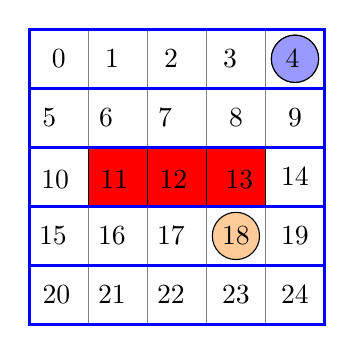
\begin{tikzpicture}[scale=1.5]
\draw[step=0.5cm,color=gray] (-1.5,-1.5) grid (1,1);
\filldraw[fill=blue,draw=black] (+0.75,+0.75) circle (0.2cm);
\filldraw[fill=red,draw=black] (0,0) rectangle (-0.5,-0.5);
\filldraw[fill=red,draw=black] (-0.5,0) rectangle (-1,-0.5);
\filldraw[fill=red,draw=black] (0,0) rectangle (0.5,-0.5);
\filldraw[fill=none,draw=blue,line width=0.4mm] (-1.5,0.5) rectangle (1,1.0);
\filldraw[fill=none,draw=blue,line width=0.4mm] (-1.5,0) rectangle (1,0.5);
\filldraw[fill=none,draw=blue,line width=0.4mm] (-1.5,-0.5) rectangle (1,0.0);
\filldraw[fill=none,draw=blue,line width=0.4mm] (-1.5,-1.0) rectangle (1,-0.5);
\filldraw[fill=none,draw=blue,line width=0.4mm] (-1.5,-1.5) rectangle (1,-1);


\filldraw[fill=blue!40!white,draw=black] (+0.75,+0.75) circle (0.2cm);
\filldraw[fill=orange!40!white,draw=black] (0.25,-0.75) circle (0.2cm);
\node at (-1.25,+0.75) {{0}};
\node at (-0.80,+0.75) {{1}};
\node at (-0.30,+0.75) {{2}};
\node at (0.20,+0.75) {{3}};
\node at (0.73,+0.75) {{4}};
\node at (-1.33,+0.25) {{5}};
\node at (-0.85,+0.25) {{6}};
\node at (-0.35,+0.25) {{7}};
\node at (0.25,+0.25) {{8}};
\node at (0.75,+0.25) {{9}};
\node at (-1.28,-0.27) {{10}};
\node at (-0.78,-0.27) {{11}};
\node at (-0.28,-0.27) {{12}};
\node at (0.28,-0.27) {{13}};
\node at (0.75,-0.25) {{14}};
\node at (-1.3,-0.75) {{15}};
\node at (-0.8,-0.75) {{16}};
\node at (-0.3,-0.75) {{17}};
\node at (0.25,-0.75) {{18}};
\node at (0.75,-0.75) {{19}};
\node at (-1.27,-1.25) {{20}};
\node at (-0.8,-1.25) {{21}};
\node at (-0.3,-1.25) {{22}};
\node at (0.25,-1.25) {{23}};
\node at (0.75,-1.25) {{24}};
\end{tikzpicture}\label{fig:simple-abstr-game-partition}}

\subfloat[Transitions from $(4,\{18\})$ in the abstract game]{
\begin{tikzpicture}[node distance=.9 cm,auto,>=latex',line join=bevel,transform shape,scale=.8]
\node at (0,0) (s0) {$(4,\{18\})$};
\node  [below left of=s0,yshift=-.2cm,xshift=-.35cm] (s2) {$(3,\{19\})$};
\node  [below right of=s0,yshift=-.2cm,xshift=.35cm] (s3) {$(9,\{Q_4,Q_5\})$};
\node  [left of=s2,xshift=-1cm] (s1) {$(3,\{Q_4,Q_5\})$};
\node  [right of=s3,xshift=1cm] (s4) {$(9,\{19\})$};

\draw [->] (s0) edge (s1.north);
\draw [->] (s0) edge (s2.north);
\draw [->] (s0) edge (s3.north);
\draw [->] (s0) edge (s4.north);
\end{tikzpicture}


\label{fig:simple-abstr-game-parttrans}}
\caption{Transitions from the initial state in the abstract game from Example~\ref{ex:simple-abstr-game}.}
\end{figure}

\bigskip                                   
\begin{eg}\label{ex:simple-abstr-game}
Consider the surveillance game from Example~\ref{ex:simple-surveillance-game}, and the abstraction partition $\part = \{Q_1,\ldots,Q_5\}$, where the set $Q_i$ corresponds to the $i$-th row of the grid as shown in Figure~\ref{fig:simple-abstr-game-partition}. We assume straight-line visibility and perfect sensing, and hence for each $l \in L$ we have $\{l\} \in \range(\obs)$.

For location $17$ of the target we have $\alpha_\part(17) = Q_4$, and for  $23$ we have $\alpha_\part(23) = Q_5$. Thus, the belief set $B = \{17,23\}$ is covered by the abstract belief set $\alpha_Q(B) = \{Q_4,Q_5\}$. Note that the set $\obs(4,17) = \obs(4,23) = \{10,15,16,17,18,20,21,22,23\}$ consists of all the locations that are not straight-line visible from location $4$.
%
The belief set $\{19\}$ is abstracted to the set $\obs(4,19) = \{19\}$.

Figure~\ref{fig:simple-abstr-game-parttrans} shows the successors of the initial state $(4,\{18\})$ of the abstract game. The concretization of the abstract belief $\{Q_4,Q_5\}$ is the set $Q_4 \cup Q_5$ of possible locations.\qed
\end{eg}

\bigskip

As explained above, there are two types of abstract belief states: those corresponding to elements of $\range(\obs)$ or to $\{l_t^{\init}\}$, and those corresponding to elements of $\mathcal P(\part)$. Abstract states in $\range(\obs)$ abstract by using the current observation (which potentially contains locations not in the current belief).
With each abstract state $(l_a,A_t)$ we can associate a set $\inabs_\part(A_t) \in \mathcal{P}(\part)$ of partitions from $\part$, that
consists of all partitions that have a non-empty intersection with $\gamma(A_t)$, that is, 
$\inabs(A_t) = \{Q \in \part \mid Q \cap \gamma(A_t) \neq \emptyset\}$. Note that if $A_t \in \mathcal P(\part)$, then we have that $\inabs_\part(A_t) = A_t$.

\bigskip

An abstract state $(l_a,A_t)$ \emph{satisfies a surveillance predicate $p_k$}, denoted $(l_a,A_t) \models p_k$, iff the number of states in the concretized belief set is less than or equal to $k$. Formally,
$$(l_a,A_t) \models p_k \Longleftrightarrow |\gamma(A_t)| \leq k.$$ Similarly, for a predicate $p \in \AP$, we define $(l_a,A_t) \models p$ iff that predicate is satisfied by all concrete states in $A_t$. Formally,
$$(l_a,A_t) \models p \Longleftrightarrow \forall l_t \in  \gamma(A_t): (l_a,l_t) \models p.$$
With these definitions, we can interpret surveillance objectives and task specifications over runs of $G_\abstr$.

Strategies (and wining strategies) for the agent and the target in an abstract belief-set game $(\alpha_\part(G),\varphi)$ are defined analogously to strategies (and winning strategies) in $G_\belief$.